\documentclass{standalone}
\usepackage{tikz}

\begin{document}
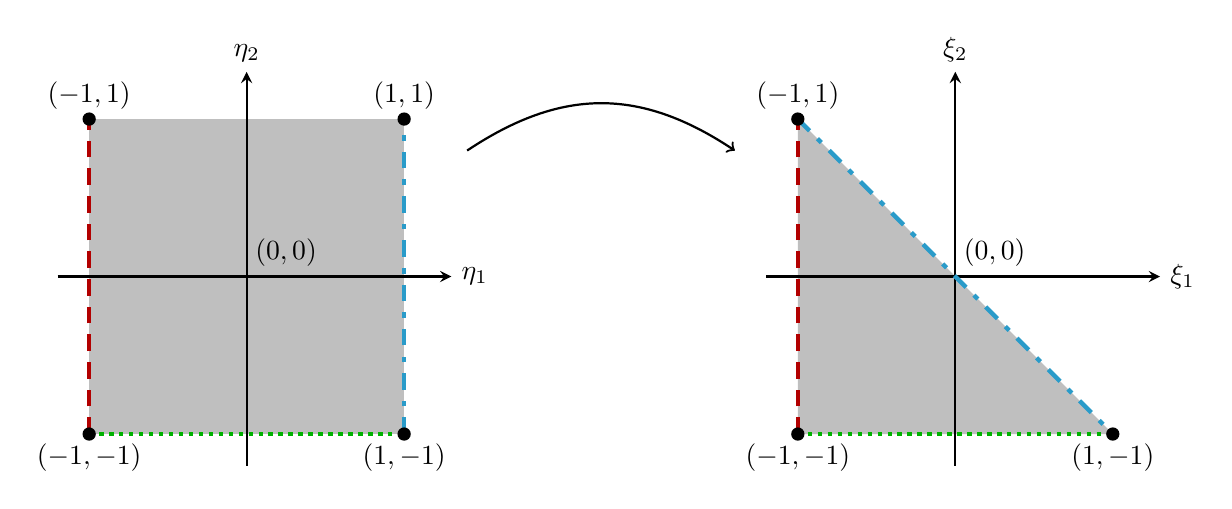
\begin{tikzpicture}[scale=2]

% --- Figure (a) ---
% Filled square
\fill[gray!50] (-1,-1) rectangle (1,1);

% Axes
\draw[-stealth,thick] (-1.2,0) -- (1.3,0) node[right] {$\eta_1$};
\draw[-stealth,thick] (0,-1.2) -- (0,1.3) node[above] {$\eta_2$};

\draw[ultra thick, red!70!black, dash pattern={on 6pt off 4pt}] (-1,-1) -- (-1,1);
\draw[ultra thick, green!70!black, dotted] (-1,-1) -- (1,-1);
\draw[ultra thick, cyan!80!black, dash pattern={on 6pt off 4pt on 2pt off 4pt}] (1,-1) -- (1,1);

% Vertices
\foreach \x/\y in {-1/-1, -1/1, 1/-1, 1/1} {
    \fill (\x,\y) circle (1.2pt);
}


% Coordinates
\node at (0.25,0.15) {$(0,0)$};
\node at (-1,1.15) {($-1,1$)};
\node at (1,1.15) {($1,1$)};
\node at (-1,-1.15) {($-1,-1$)};
\node at (1,-1.15) {($1,-1$)};



% --- Figure (b) ---
\begin{scope}[xshift=4.5cm]
    % Filled triangle
    \fill[gray!50] (-1,-1) -- (-1,1) -- (1,-1) -- cycle;
    


    % Axes
    \draw[-stealth,thick] (-1.2,0) -- (1.3,0) node[right] {$\xi_1$};
    \draw[-stealth,thick] (0,-1.2) -- (0,1.3) node[above] {$\xi_2$};
    
		\draw[ultra thick, red!70!black, dash pattern={on 6pt off 4pt}] (-1,-1) -- (-1,1);
		\draw[ultra thick, green!70!black, dotted] (-1,-1) -- (1,-1);
		\draw[ultra thick, cyan!80!black, dash pattern={on 6pt off 4pt on 2pt off 4pt}] (-1,1) -- (1,-1);

		% Vertices
    \foreach \x/\y in {-1/-1, -1/1, 1/-1} {
        \fill (\x,\y) circle (1.2pt);
    }

    % Coordinates
    \node at (0.25,0.15) {$(0,0)$};
    \node at (-1,1.15) {($-1,1$)};
    \node at (1,-1.15) {($1,-1$)};
    \node at (-1,-1.15) {($-1,-1$)};
\end{scope}

% --- Curved arrow between figures ---
\draw[->,thick] (1.4,0.8) .. controls (2.0,1.2) and (2.5,1.2) .. (3.1,0.8);

\end{tikzpicture}
\end{document}

